\documentclass[11pt, a4paper]{article}

\usepackage{style}

\author{Vladislav Mlejnecký}

\title{%
  Číslicové zpracování signálů\\
  \large Úloha číslo 7.\\
  Aplikace filtrů - simulace pomocí Matlab - II}

\begin{document}

    \maketitle
    
    \section{Zadání}
        \begin{enumerate}
            \item
            Vygenerujte signál o délce 512 vzorků složený ze základního kmitočtu a dalších dvou
            harmonických složek průběhu, přidejte rušivý signál harmonického průběhu, který bude od
            druhé harmonické posunut o 100Hz výše. Nakreslete spektrum signálu.
            \item
            Navrhněte filtr, kterým přidaný signál odfiltrujete. Postupně volíme aproximace
            butterworth, čebyševI, čebyševII a eliptická, kontrolujeme výsledné rozložení nul a pólů
            \item
            Aplikujte navržený filtr na složený signál – funkce „filter“ v Matlabu
            \item
            Zobrazujeme graficky spektrum původního signál sestávající ze tří složek, dále signál
            s přidaným posunutým kmitočtem a výsledek po filtraci.
            Zvolte:
            \begin{itemize}
                \item vzorkovací kmitočet 10000Hz
                \item N=512 vzorků
                \item kmitočet signálu = 1100Hz
            \end{itemize}
            \item
            K signálu dle bodu 1. přidejte další signál, tentokrát poblíž 3. harmonické a posunutý rovněž
            o 100Hz. Dále postupujte obdobně bodům 2. až 4.
            \item
            Nakreslete kmitočtovou charakteristiku výsledného filtru (součin polynomů funkce conv()).
        \end{enumerate}
                
    \section{Výsledné grafy}
    
        \subsection{Charakteristiky filtrů}
        
            \begin{figure}[H]
                \centering
                \begin{minipage}{.5\textwidth}
                    \centering
                    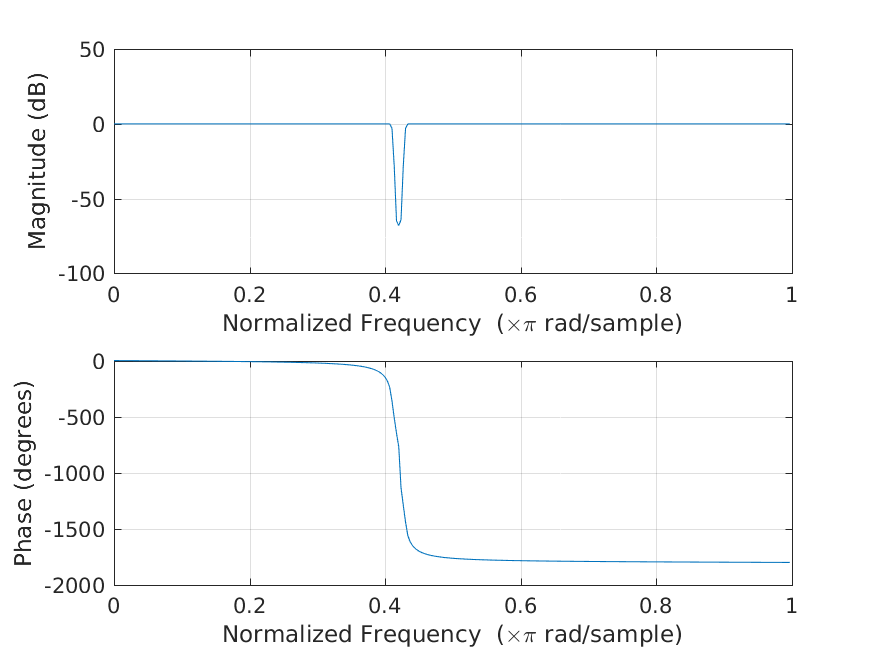
\includegraphics[width=.9\textwidth]{matlab/first.png}
                    \caption{První filtr}
                    \label{fig:freqz1}
                \end{minipage}%
                \begin{minipage}{.5\textwidth}
                    \centering
                    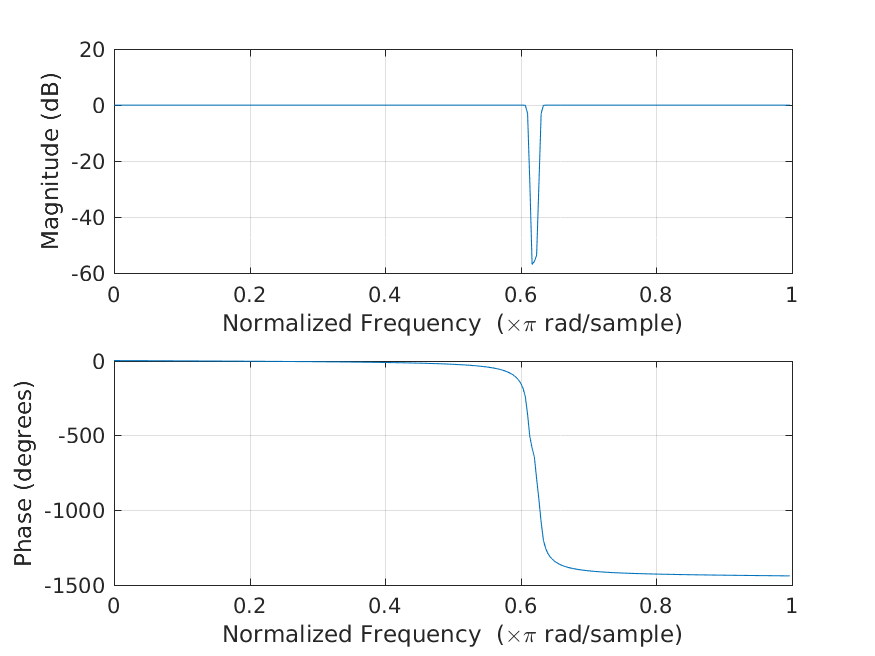
\includegraphics[width=.9\textwidth]{matlab/second.png}
                    \caption{Druhý filtr}
                    \label{fig:freqz2}
                \end{minipage}
            \end{figure}
            
        \subsection{Původní signály}
    
            \begin{figure}[H]
                \centering
                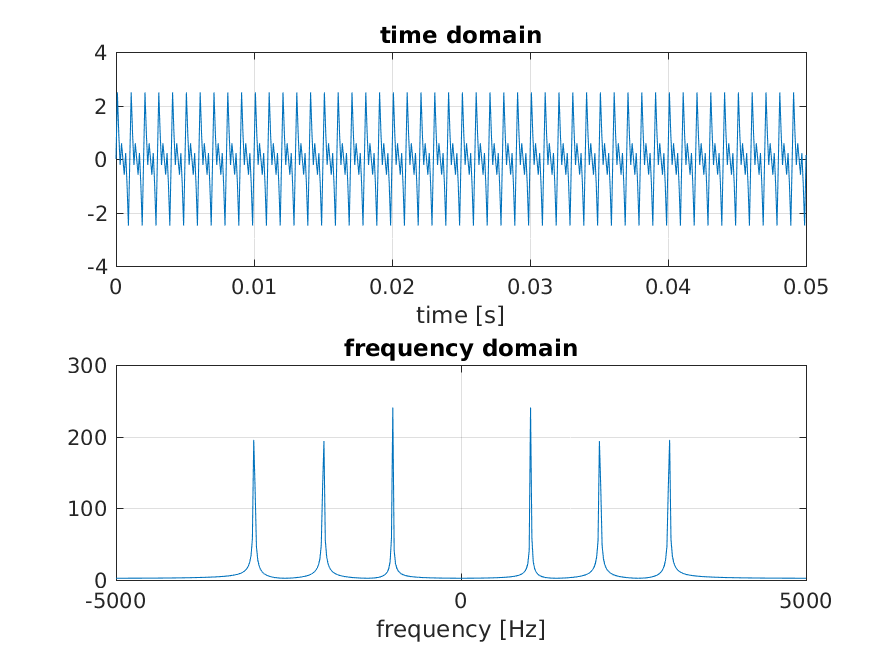
\includegraphics[width=.5\textwidth]{matlab/orig.png}
                \caption{Průběh a spektrum čistého signálu}
                \label{fig:orig}
            \end{figure}
    
            \begin{figure}[H]
                \centering
                \begin{minipage}{.5\textwidth}
                    \centering
                    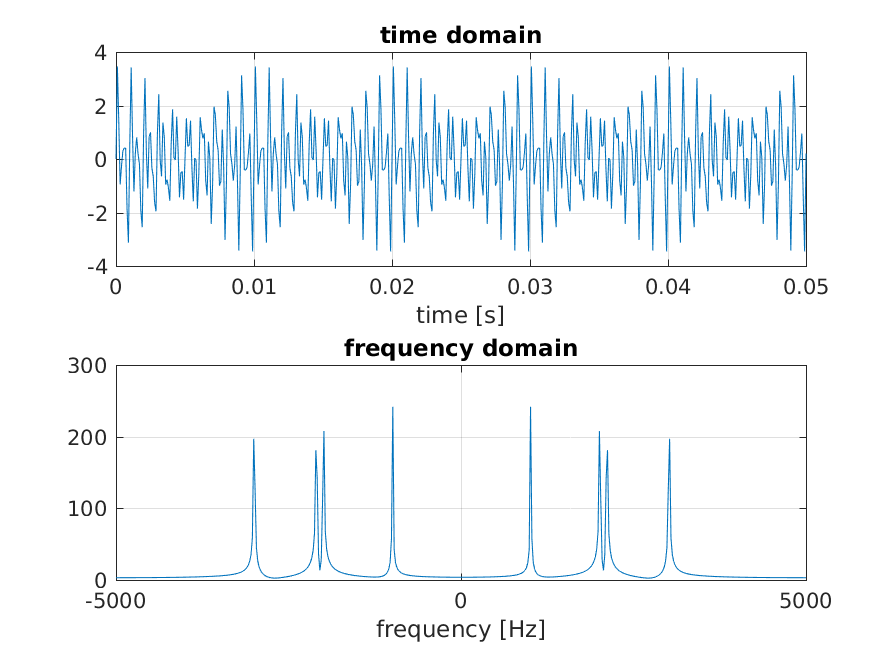
\includegraphics[width=.9\textwidth]{matlab/y1.png}
                    \caption{Spektrum signálu A}
                    \label{fig:y1}
                \end{minipage}%
                \begin{minipage}{.5\textwidth}
                    \centering
                    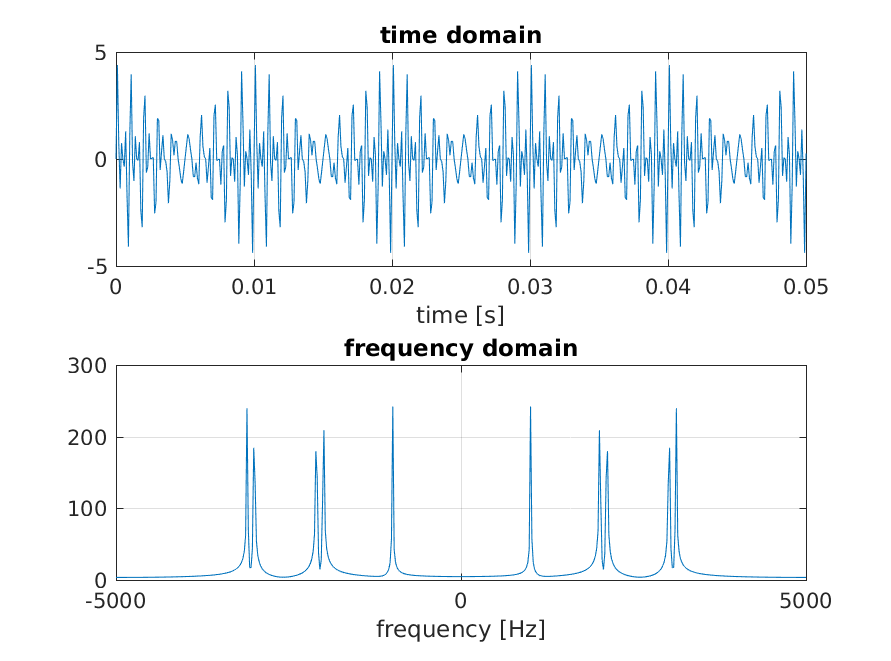
\includegraphics[width=.9\textwidth]{matlab/y2.png}
                    \caption{Spektrum signálu B}
                    \label{fig:y2}
                \end{minipage}
            \end{figure}
            
        \subsection{Filtrované signály}
        
            \begin{figure}[H]
                \centering
                \begin{minipage}{.5\textwidth}
                    \centering
                    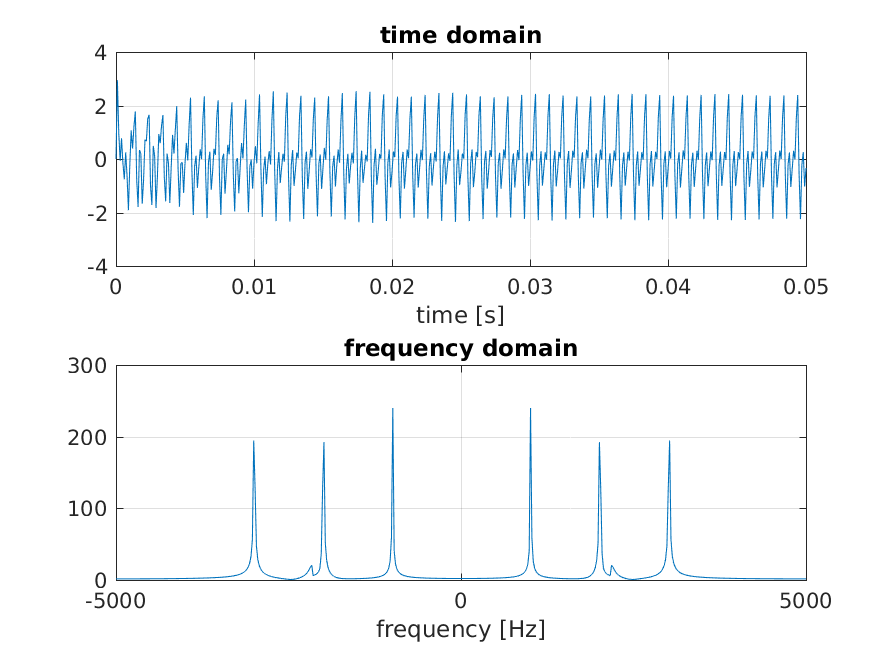
\includegraphics[width=.9\textwidth]{matlab/y1_clean.png}
                    \caption{Spektrum signálu A po filtraci}
                    \label{fig:y1_clean}
                \end{minipage}%
                \begin{minipage}{.5\textwidth}
                    \centering
                    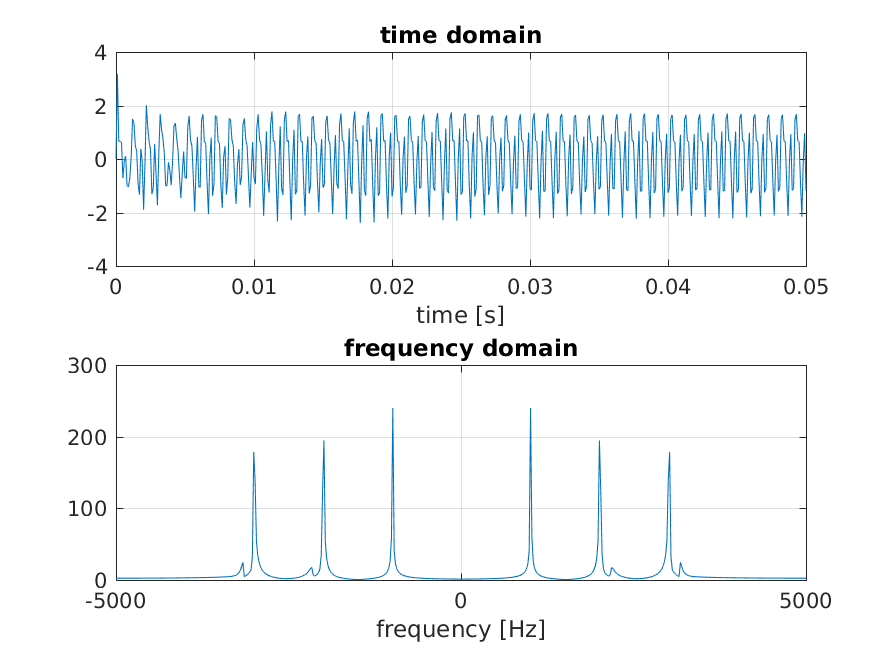
\includegraphics[width=.9\textwidth]{matlab/y2_clean.png}
                    \caption{Spektrum signálu B po filtraci}
                    \label{fig:y2_clean}
                \end{minipage}
            \end{figure}
        
    
    \section{Komentář k výsledkům}
    
        Původní signál v časové i frekvenční oblasti lze vidět na 
        obrázku \ref{fig:orig}. Po přidání nežádoucích signálu o 
        frekvenci $F_A = 2100 Hz$ a $F_B = 3100 Hz$, vznikli signály 
        které je možné vidět na obrázcích \ref{fig:y1} a \ref{fig:y2}. 
        
        Pro odfiltrování byli navrženy dva filtry typu pásmová zádrž 
        osmého stupně s aproximací \textit{butter}. Zlomové frekvence 
        prvního filtru jsou $F_{A1} = 2050 Hz$ a $F_{A2} = 2150 Hz$. 
        Zlomové frekvence druhého filtru pak jsou $F_{B1} = 3050 Hz$ a 
        $F_{B2} = 3150 Hz$.
        
        Vstupní signály jsou filtrovány navrženými filtry, první signál 
        pouze prvním filtrem, druhý signál prvním filtrem a následně i 
        druhým filtrem. To odpovídá situaci kdy jsou filtry zapojeny v 
        kaskádě.
        
        Výsledné vyfiltrované signály jsou zachyceny na obrázcích 
        \ref{fig:y1_clean} a \ref{fig:y2_clean}.
                    
                    
    \section{Výpis zdrojového kódu}
    
\begin{lstlisting}[language=matlab, frame=single] 
Fs = 10000;
t = 0:1/Fs:511/Fs;

%create original signal
y_orig = sin(2 * pi * 1000 * t); 
y_orig = y_orig + sin(2 * pi * 2000 * t); 
y_orig = y_orig + sin(2 * pi * 3000 * t);

%add another signals
y1 = y_orig + sin(2 * pi * 2100 * t);
y2 = y1 + sin(2 * pi * 3100 * t);

%calculate two filters
Fst1 = [2050 2150];
Fst2 = [3050 3150];
[b1,a1] = butter(8, (2/Fs) .* Fst1  , 'stop'); 
[b2,a2] = butter(8, (2/Fs) .* Fst2  , 'stop'); 

%filter first signal
y1_clean = filter(b1,a1,y1);

%filter second signal
y2_clean = filter(b1, a1, y2);
y2_clean = filter(b2, a2, y2_clean);

%print results
make_fft_graph(y_orig, t, Fs, 'orig');
make_fft_graph(y1, t, Fs, 'y1');
make_fft_graph(y2, t, Fs, 'y2');
make_fft_graph(y1_clean, t, Fs, 'y1_clean');
make_fft_graph(y2_clean, t, Fs, 'y2_clean');

function make_fft_graph(y, t, Fs, FileName)
    %calculate FFT
    y_spec = fft(y);
    y_spec=abs(fftshift(y_spec));
    f_spec = Fs/2 * linspace(-1, 1, length(y));
    
    %draw a graph
    h = figure();
    subplot(2, 1, 1);
    plot(t,y);
    title('time domain');
    xlabel('time [s]');
    grid on;
    a = axis;
    axis([0 0.05 a(3) a(4)]);
    subplot(2, 1, 2);
    plot(f_spec, y_spec);
    title('frequency domain');
    xlabel('frequency [Hz]');
    grid on;
    
    saveas(h, [FileName '.png']);
    close(h);
    clear h;
end
\end{lstlisting}

\end{document}

